%! TEX program = LuaTeX

\documentclass[nobackground,dvipsnames,table,aspectratio=169]{beamer}
\usepackage{cs152}

\mode<presentation>
{\usetheme{Hannover}
    \usecolortheme{cs152}
    \setbeamercovered{transparent}
    \useinnertheme[shadow=false]{rounded}
    \usebackgroundtemplate{}
    \setbeamercolor*{frametitle}{parent=palette primary}
    \setbeamerfont{block title}{size={}}
    \setbeamertemplate{navigation symbols}{}
}

\title{Child and Adult Sexual Exploitation 2: Sextortion and NCII}
\subtitle{CS 152 --- Lecture 10}

\author[A. Stamos]{Alex Stamos}
\institute[Stanford University]{Stanford Cyber Policy Center}
\date[2022]{\today}
\subject{CS 152 --- Trust and Safety Engineering}
%\titlegraphic{
\includegraphics[width=5cm]{img/cyber-logo-white-black-red-WEB}}

% Change the level of bulleting on the ToC page
\setcounter{tocdepth}{2}

\graphicspath{{img/lesson10}}

\begin{document}

\begin{frame}
    \titlepage
\end{frame}

%\begin{frame}{} %TODO
%    \thispagestyle{empty}
%    \AddToShipoutPictureBG*{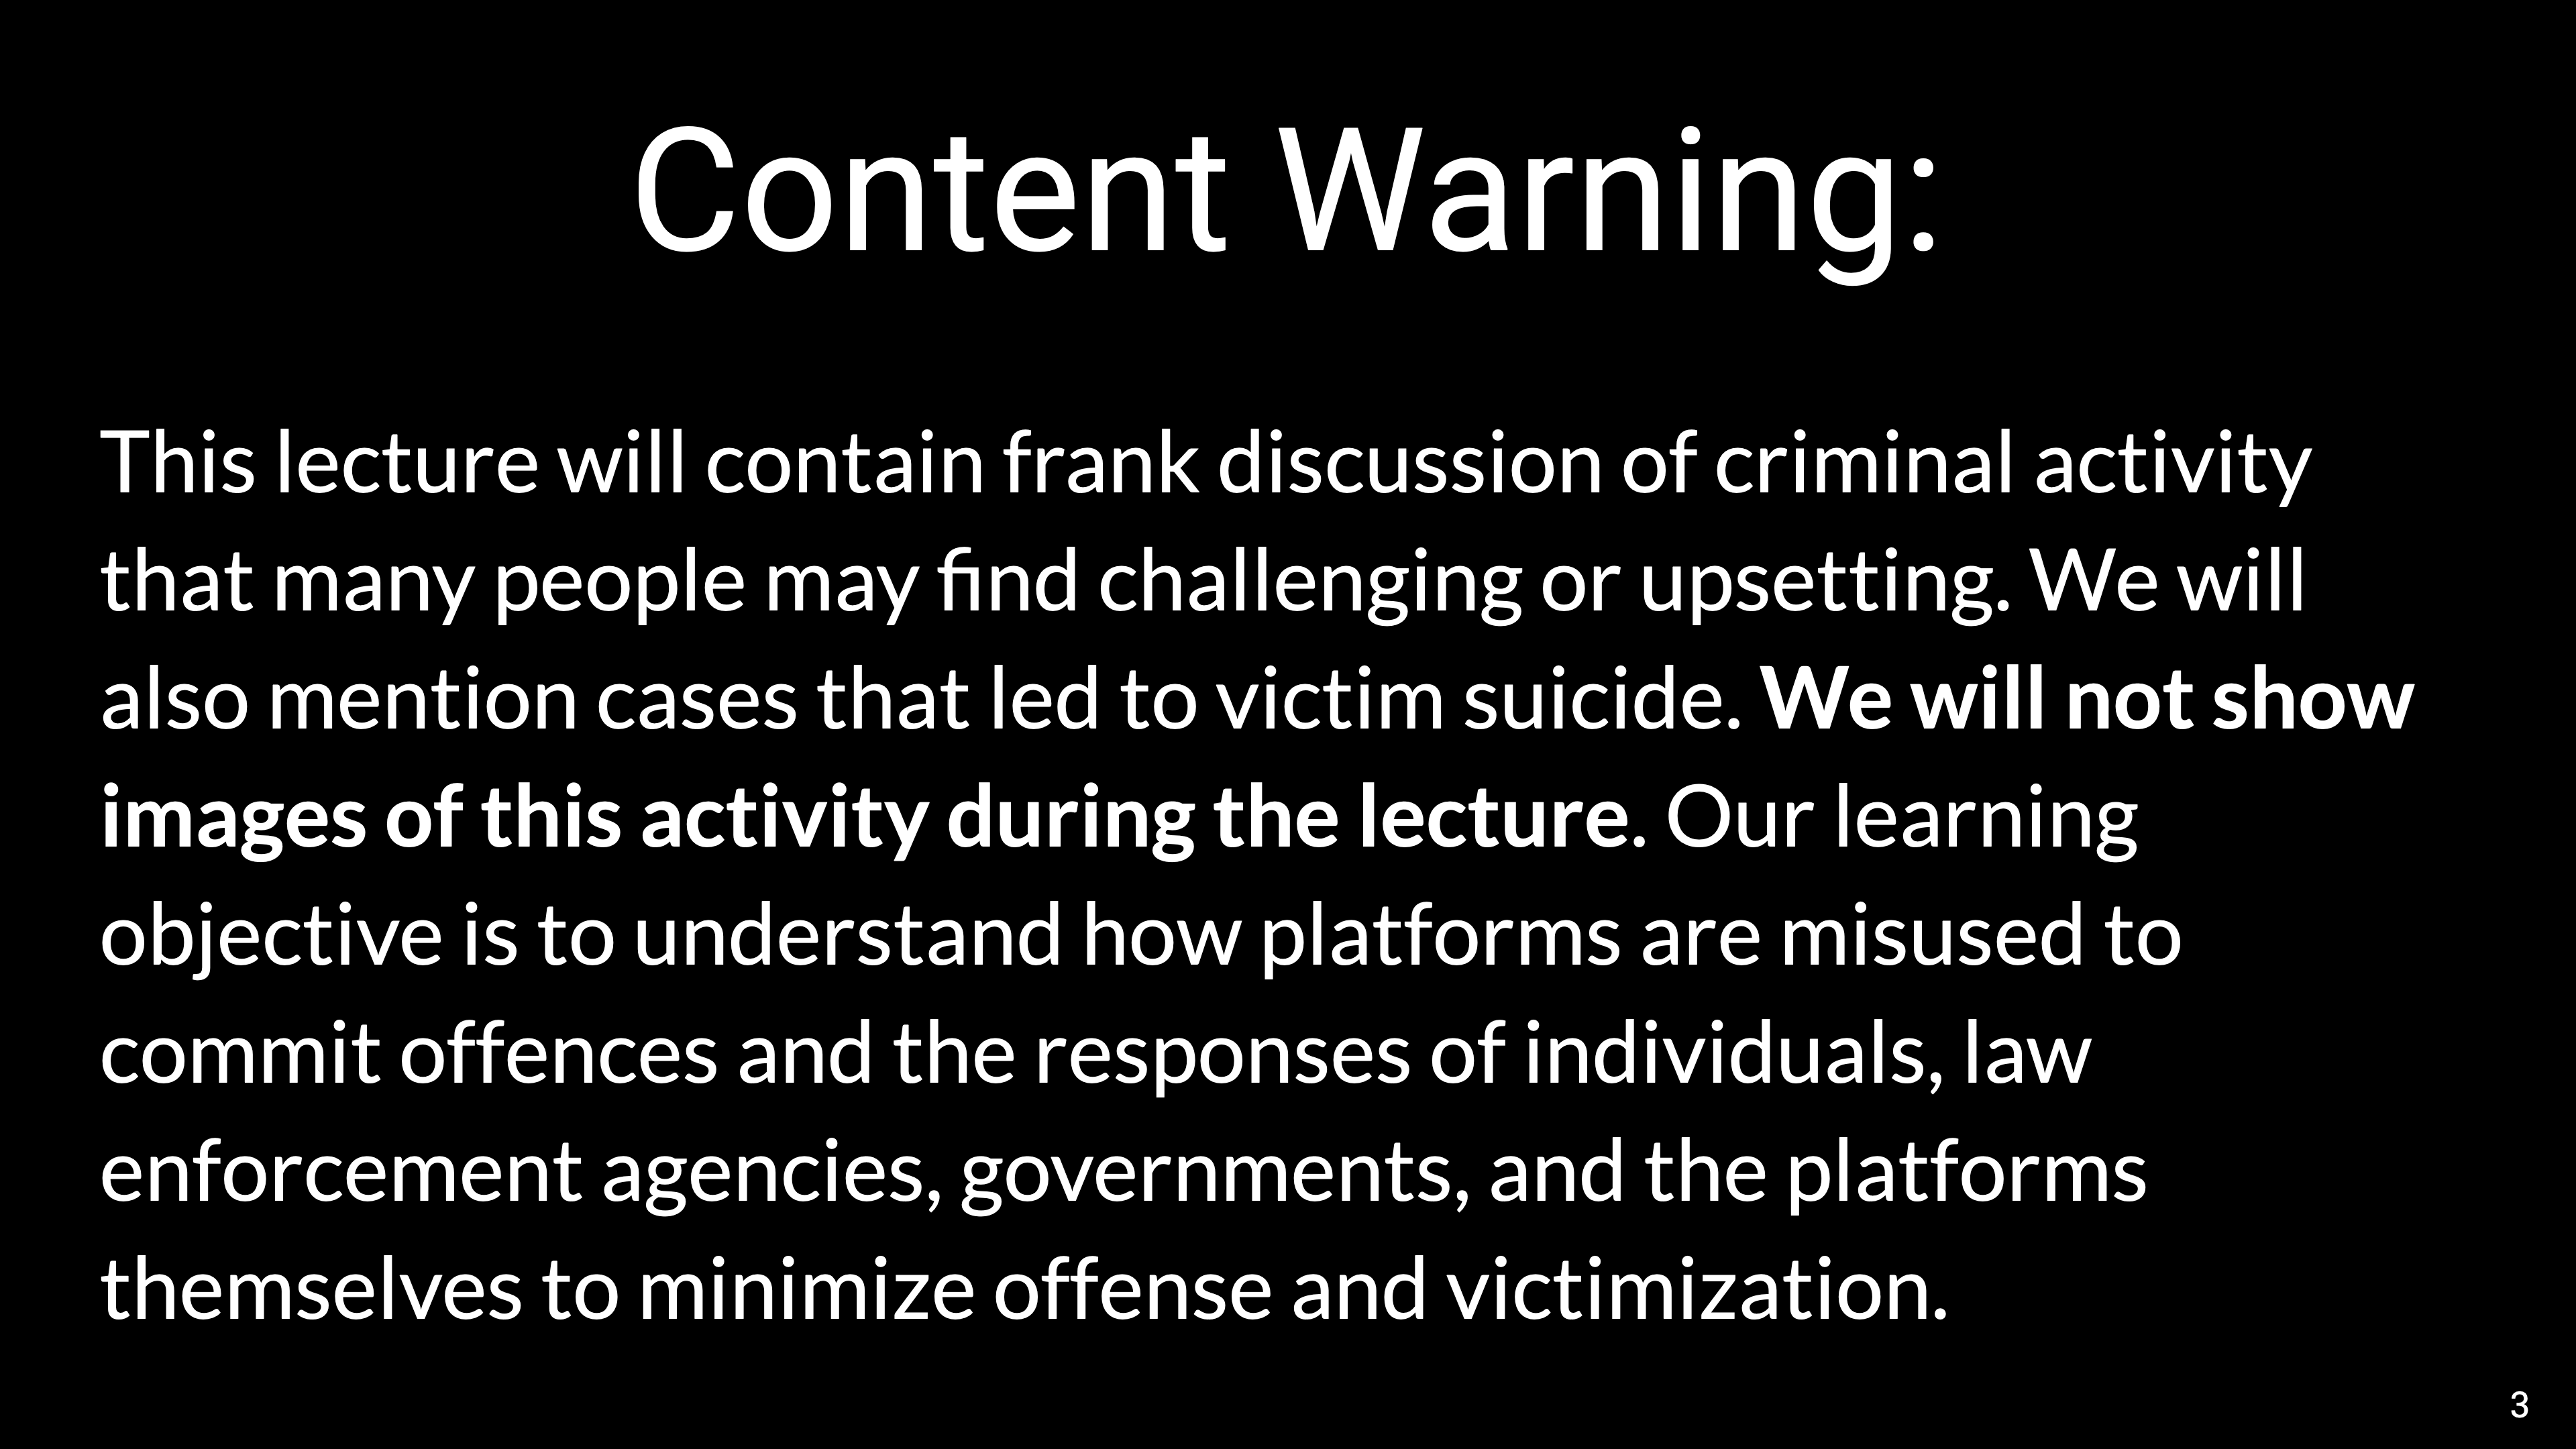
\includegraphics[with=\paperwidth]{content-warning}}
%\end{frame}

\section{Case Study: Amanda Todd}

\begin{frame}{Case Study: Amanda Todd}
    \begin{columns}
        \column{0.5\textwidth}
            %TODO image
        \column{0.5\textwidth}
            \begin{itemize}
                \item 2012: took her own life after 2-3 years of blackmail and harassment (sextortion)
                \item Suspect traced to The Netherlands
                \item Prosecuted for 72 offences against 39 victims
                \item Initial sentence in NL: 10 yrs & 8 mths
            \end{itemize}
    \end{columns}
\end{frame}

\begin{frame}{Family Advocacy}
    %TODO image
    \begin{columns}
        \column{0.55\textwidth}
            %TODO image
        \column{0.45\textwidth}
            %TODO image
    \end{columns}
\end{frame}

\begin{frame}{Family Advocacy}
    %TODO 2 images
\end{frame}

\section{What Will We Discuss Today?}

\begin{frame}{What Will We Discuss Today?}
    \large
    \begin{itemize}
        \item Taxonomy of Non-Consensual Intimate Imagery (NCII)
        \item How predators use technology to groom and traffic children
        \item Prevalence of sextortion and impacts on victims
        \item Modern responses to grooming, sextortion, and new imagery
    \end{itemize}
\end{frame}

\section{NCII}

\begin{frame}{NCII:}
    \centering
    \LARGE
    \textit{\underline{N}on-\underline{C}onsensual \underline{I}ntimate \underline{I}mages}
\end{frame}

\begin{frame}{Definitions}
    \large
    \begin{itemize}
        \item \textbf{Grooming:} creating a relationship with a child/young person  to earn their trust and then exploit and/or abuse them
        \item \textbf{Sextortion:} when offender threatens to distribute target’s  images/videos of a sexual nature unless they provide them with money or sexual favors
    \end{itemize}
\end{frame}

\section{Taxonomy of NCII}

\begin{frame}{NCII Taxonomy (Adults and Children)}
    %TODO diagram
\end{frame}

\begin{frame}{Power as a Motivator}
    %TODO image
\end{frame}

\section{How NCII Happens}

\begin{frame}{NCII Taxonomy: Ex-Partner Distribution}
    %TODO diagram
\end{frame}

\begin{frame}{How NCII Happens: Ex-Partner Scenario}
    %TODO diagram 1
\end{frame}

\begin{frame}{How NCII Happens: Ex-Partner Scenario}
    %TODO diagram 2
\end{frame}

\begin{frame}{How NCII Happens: Ex-Partner Scenario}
    %TODO diagram 3
\end{frame}

\begin{frame}{How NCII Happens: Ex-Partner Scenario}
    %TODO diagram 4
\end{frame}

\begin{frame}{Ex-Partner and Political Blackmail}
    \begin{columns}
        \column{0.4\textwidth}
            %TODO image
        \column{0.6\textwidth}
            %TODO images
    \end{columns}
\end{frame}

\begin{frame}{NCII Taxonomy: Sextortion for Money}
    %TODO diagram
\end{frame}

\begin{frame}{How NCII Happens - Sextortion for Money Scenario}
    %TODO diagram 1
\end{frame}

\begin{frame}{How NCII Happens - Sextortion for Money Scenario}
    %TODO diagram 2
\end{frame}

\begin{frame}{How NCII Happens - Sextortion for Money Scenario}
    %TODO diagram 3
\end{frame}

\begin{frame}{How NCII Happens - Sextortion for Money Scenario}
    %TODO diagram 4
\end{frame}

\begin{frame}{How NCII Happens - Sextortion for Money Scenario}
    %TODO diagram 5
\end{frame}

\begin{frame}{Case Study: CS152 Student}
    \begin{columns}
        \column{0.3\textwidth}
            %TODO images
        \column{0.7\textwidth}
            \begin{itemize}
                \item Took CS152 
                \item Met “Sophia” on Tinder
                \item Talk for 3 days-set up a skype
                \item She has no camera-> begins masturbating and encourages him to do the same
                \item Demanded money or send video to “everyone”
            \end{itemize}
    \end{columns}
\end{frame}

\begin{frame}{Case Study: Daniel Perry}
    \begin{columns}
        \column{0.4\textwidth}
            %TODO image
        \column{0.6\textwidth}
            \begin{itemize}
                \item 2013: started chatting with a girl on Skype
                \item Minutes after being blackmailed for money he took his own life at age 17
                \item Suspect was identified as a male based in the Philippines
            \end{itemize}
    \end{columns}
\end{frame}

\begin{frame}{Standing Up to Financial Sextortion}
    %TODO images
    \begin{columns}
        \column{0.5\textwidth}
        \column{0.5\textwidth}
    \end{columns}
\end{frame}

\begin{frame}{NCII Taxonomy: Hacker Distribution}
    %TODO diagram
\end{frame}

\begin{frame}{How NCII Happens - Hack Scenario}
    %TODO diagram 1
\end{frame}

\begin{frame}{How NCII Happens - Hack Scenario}
    %TODO diagram 2
\end{frame}

\begin{frame}{How NCII Happens - Hack Scenario}
    %TODO diagram 3
\end{frame}

\begin{frame}{How NCII Happens - Hack Scenario}
    %TODO diagram 4
\end{frame}

\begin{frame}{How NCII Happens - Hack Scenario}
    %TODO diagram 5
\end{frame}

\begin{frame}{Anyone Can Be a Victim, Motivation Is Rarely Revenge/Manipulation}
    \begin{columns}
        \column{0.4\textwidth}
            \begin{columns}
                \column{0.5\textwidth}
                    %TODO image
                \column{0.5\textwidth}
                    %TODO image
            \end{columns}
            %TODO image
        \column{0.6\textwidth}
            %TODO 2 images
    \end{columns}
\end{frame}

\begin{frame}{Case Study: Jeff Bezos}
    \begin{columns}
        \column{0.4\textwidth}
            %TODO image
        \column{0.6\textwidth}
            %TODO image
            “Any personal embarrassment AMI could cause me takes a back seat because there’s a much more important matter involved here. If in my position I can’t stand up to this kind of extortion, how many people can? (On that point, numerous people have contacted our investigation team about their similar experiences with AMI, and how they needed to capitulate because, for example, their livelihoods were at stake.”)
    \end{columns}
\end{frame}

\begin{frame}{NCII Taxonomy - 'Sextortion' for Content}
    %TODO diagram
\end{frame}

\begin{frame}{}
    “Sextortion is by far the most significantly growing threat to children...\href{https://www.justice.gov/psc/file/842411/download}{more than 60\% of survey respondents} indicated this type of online enticement of minors was increasing.”
    %TODO image
\end{frame}

\begin{frame}{Remember This: How Does CSE Manifest Online?}
    %TODO image
    [Baines (2018)]
\end{frame}

\begin{frame}{Modern Day: Social Media, Livestream Abuse, and Video Games}
    %TODO image
\end{frame}

\begin{frame}{Leveraging Multiple Technologies and Platforms }
    \begin{columns}
        \column{0.4\textwidth}
            %TODO diagram
        \column{0.4\textwidth}
            \begin{itemize}
                \item Social and gaming platforms are used to make initial contact.
                \item Children may then be encouraged to move to less open/more secure messaging apps.
                \item Children may be groomed to share sexual images/videos they have taken themselves.
                \item This can rapidly develop into the sextortion blackmail scenario.
                \item Children may also be groomed for offline meets for sexual activity.
            \end{itemize}
    \end{columns}
\end{frame}

\begin{frame}{Video Games as "Hunting Grounds"}
    %TODO image
\end{frame}

\begin{frame}{Evolution & Complexity - “Live Streaming” Example}
    %TODO diagram
\end{frame}

\section{Prevalence and Impact}

\begin{frame}{NCII Prevalence}
    \begin{columns}
        \column{0.4\textwidth}
            %TODO image
        \column{0.6\textwidth}
            \begin{itemize}
                \item 61\% said they had shared nude photos/video with someone else
                \item 23\% were victims of revenge porn, 90\% of victims were women
                \item Posted by:
                \begin{itemize}
                    \item 57\% ex-boyfriend
                    \item 6\% ex-girlfriend
                    \item 23\% ex-friend
                    \item 7\% friend
                    \item 7\% family member
                \end{itemize}
            \end{itemize}
            \textit{Results sampled from visitors to website, so probably overstates prevalence}
    \end{columns}
\end{frame}

\begin{frame}{NCII Platforms}
    %TODO image
\end{frame}

\begin{frame}{NCII Impact}
    \begin{columns}
        \column{0.4\textwidth}
            %TODO image
        \column{0.6\textwidth}
            \begin{itemize}
                \item 93\% of victims said they have suffered significant emotional distress due to being a victim
                \item 82\% said they suffered significant impairment in social, occupational, or other important areas of functioning due to being a victim
                \item 34\% said that being a victim has jeopardized their relationships with family
                \item 49\% said they have been harassed or stalked online by users that have seen their material
                \item 30\% said they have been harassed or stalked outside of the Internet (in person, over the phone) by users that have seen the material online
            \end{itemize}
    \end{columns}
\end{frame}

\section{Responses and Mitigations}

\begin{frame}{Policy Responses}
    \large
    \begin{enumerate}
        \item Create detailed policies for various forms of NCII
        \item Have investigatory teams that work with law enforcement
        \item Enlist lawyers and policy teams who understand this area
        \item Invest in coordinating bodies
        \item Publish transparency reports on NCII/grooming/trafficking
        \item Create resiliency programs for employees working on these issues
        \item Public awareness and education
    \end{enumerate}
\end{frame}

\begin{frame}{Responding to CSE}
    \centering
    %TODO image
    [Baines (2018)]
\end{frame}

\begin{frame}{NCII and the Law}
    \large
    \begin{itemize}
        \item Is it a sexual offence?
        \item Is it a privacy violation?
    \end{itemize}
\end{frame}

\begin{frame}{Sextortion Is Not Criminalized Under U.S. Federal Law}
    \begin{columns}
        \column{0.3\textwidth}
            Prosecutors rely on other charges:
            \begin{itemize}
                \item 18 USC 875: criminalizes interstate extortion
                \item Stalking
                \item CSE/CSAM production, distribution, and/or possession
            \end{itemize}
        \column{0.7\textwidth}
            %TODO image
    \end{columns}
\end{frame}

\begin{frame}{Criminalizing NCII - A Timeline [Franks (2015)]}
    \begin{itemize}
        \item In 2009, the \textbf{Philippines} became the first country to criminalize nonconsensual pornography, with a penalty of up to 7 years’ imprisonment.
        \item The Australian state of \textbf{Victoria} outlawed non-consensual pornography in 2013.
        \item In 2014, \textbf{Israel} became the first country to classify non-consensual pornography as sexual assault, punishable by up to 5 years imprisonment. Canada criminalized the conduct the same year.
        \item Also in 2014, a \textbf{German} court ruled that an ex-partner must delete intimate images of his former partner upon request.
        \item \textbf{England and Wales} criminalized the conduct in February 2015. \textbf{New Zealand} followed in July 2015.
        \item According to a \href{https://www.internetlab.org.br/wp-content/uploads/2018/11/Fighting_the_Dissemination_of_Non.pdf}{2018 study}, \textbf{11 countries} have specific laws against the dissemination of NCII and \textbf{21 countries} have other/general laws.
        \item Before 2013, only three \textbf{U.S. states} – New Jersey, Alaska, and Texas – had criminal laws directly applicable to NCII. Today, 46 STATES + DC + one territory now have NCII laws [Cyber Civil Rights Initiative]. 42 STATES + DC have laws on “revenge porn.”
    \end{itemize}
\end{frame}

\begin{frame}{Education and Awareness}
    \centering
    \begin{columns}
        \column{0.5\textwidth}
            %TODO image
        \column{0.5\textwidth}
            %TODO image
    \end{columns}
\end{frame}

\begin{frame}{}
    \thispagestyle{empty}
    %TODO
\end{frame}

\begin{frame}{Product/Technical Responses}
    \large
    \begin{enumerate}
        \item Preemptive removal of known and unknown photos/videos
        \item Empathetic reporting flows
        \item Flag potential grooming behaviors via proactive scanning
        \item Enforce identity indicators around age
        \item Restrict discovery of children by unfamiliar adults
    \end{enumerate}
\end{frame}

\begin{frame}{Proactive Detection}
    %TODO image
\end{frame}

\begin{frame}{Prevention Mechanisms - Facebook}
    \centering
    Pre-emptive reporting of images
    %TODO image
    \url{https://www.facebook.com/safety/notwithoutmyconsent/pilot}
\end{frame}

\begin{frame}{The Response}
    %TODO 2 images
\end{frame}

\begin{frame}{Reporting and Takedown}
    \begin{columns}
        \column{0.5\textwidth}
            %TODO image
            \url{https://www.cybercivilrights.org/online-removal/}
        \column{0.5\textwidth}
            %TODO image
    \end{columns}
\end{frame}

\begin{frame}{NCII Reporting - Microsoft}
    %TODO image
\end{frame}

\begin{frame}{NCII Reporting - Facebook}
    %TODO Image
\end{frame}

\begin{frame}{The Pornhub Case}
    \begin{columns}
        \column{0.5\textwidth}
            \begin{itemize}
                \item NYT article shed light on distribution of NCII on PornHub
                \item MindGeek, PornHub’s parent company, changed policies:
                \begin{itemize}
                    \item Prevented download of videos
                    \item Implemented restrictions on who could upload content
                    \item Took down millions of videos uploaded by unverified users
                \end{itemize}
                \item Visa and MasterCard banned the use of their cards on Pornhub
            \end{itemize}
        \column{0.5\textwidth}
            %TODO image
    \end{columns}
\end{frame}

\section{What's Next?}

\begin{frame}{Deepfakes, AR/VR NCII, and Consent?}
    \begin{columns}
        \column{0.4\textwidth}
            %TODO image
        \column{0.4\textwidth}
            %TODO image
    \end{columns}
\end{frame}

\begin{frame}{VR and the Metaverse}
    %TODO image
\end{frame}

\begin{frame}{Encryption}
    %TODO image
\end{frame}

\begin{frame}{Increasing Focus on Liability of Platforms}
    %TODO Image
    Source: BBC News
\end{frame}

\begin{frame}{Additional OPEN QUESTIONS}
    \begin{columns}
        \column{0.45\textwidth}
            %TODO 2 images
        \column{0.55\textwidth}
            \begin{itemize}
                \item Current responses rely on \textbf{US platforms dominating.} What if this doesn’t continue?
                \item \textbf{e2e encryption} & CSAM detection 
                \item \textbf{Social VR/AR/MR:} Emotional impact of “co-presence” is greater
                \item \textbf{Haptics:} physical assault via online platforms?
            \end{itemize}
    \end{columns}
\end{frame}

\end{document}